\section*{Anexos}
\addcontentsline{toc}{section}{Anexos}

\subsection*{Árbol de problemas}
\addcontentsline{toc}{subsection}{Árbol de problemas}

\textbf{Problema Principal:}

\vspace{0.3cm}
Detección tardía del riesgo de shock hemorrágico en pacientes sometidos a cirugía mayor no cardiaca postoperatoria

\vspace{0.5cm}
\textbf{Causas:}

\begin{itemize}
    \item \textbf{Causa 1: Dependencia exclusiva de la experiencia médica}
    \begin{itemize}
        \item Sub-causa 1: Variabilidad en la interpretación clínica
        \begin{itemize}
            \item Sub-sub-causa 1: Diferencias en criterios diagnósticos entre profesionales
            \item Sub-sub-causa 2: Falta de protocolos estandarizados de evaluación
        \end{itemize}
        \item Sub-causa 2: Sesgos cognitivos en la toma de decisiones clínicas
        \item Sub-causa 3: Limitaciones humanas en el monitoreo continuo
        \begin{itemize}
            \item Sub-sub-causa 1: Fatiga del personal médico durante procedimientos prolongados
            \item Sub-sub-causa 2: Dificultad para detectar cambios sutiles en signos vitales
            \item Sub-sub-causa 3: Sobrecarga de información durante situaciones críticas
        \end{itemize}
    \end{itemize}
    
    \item \textbf{Causa 2: Protocolos clínicos no actualizados}
    \begin{itemize}
        \item Sub-causa 1: Enfoque reactivo en lugar de predictivo
        \item Sub-causa 2: Criterios diagnósticos basados en manifestaciones tardías
        \item Sub-causa 3: No consideración de factores de riesgo individuales
    \end{itemize}
    
    \item \textbf{Causa 3: Escasa personalización según características del paciente}
    \begin{itemize}
        \item Sub-causa 1: Ignorancia de comorbilidades específicas
        \item Sub-causa 2: Falta de adaptación a características demográficas
    \end{itemize}
\end{itemize}

\vspace{0.5cm}
\textbf{Efectos:}

\begin{itemize}
    \item \textbf{Efecto 1: Aumento de la mortalidad postoperatoria}
    \begin{itemize}
        \item Sub-efecto 1: Muertes por hemorragia no controlada
        \item Sub-efecto 2: Daño irreversible a órganos por hipoperfusión prolongada
        \item Sub-efecto 3: Mayor riesgo de infecciones postoperatorias
        \item Sub-efecto 4: Falla multiorgánica por manejo tardío
    \end{itemize}
    
    \item \textbf{Efecto 2: Mayor necesidad de transfusiones sanguíneas}
    \begin{itemize}
        \item Sub-efecto 1: Uso ineficiente de recursos sanguíneos
        \begin{itemize}
            \item Sub-sub-efecto 1: Transfusiones reactivas en lugar de preventivas
            \item Sub-sub-efecto 2: Escasez de hemoderivados en momentos críticos
            \item Sub-sub-efecto 3: Mayor riesgo de reacciones adversas
        \end{itemize}
        \item Sub-efecto 2: Complicaciones asociadas a transfusiones
        \begin{itemize}
            \item Sub-sub-efecto 1: Sobrecarga circulatoria
            \item Sub-sub-efecto 2: Reacciones inmunológicas
            \item Sub-sub-efecto 3: Mayor riesgo de infecciones
        \end{itemize}
    \end{itemize}
    
    \item \textbf{Efecto 3: Incremento de complicaciones postoperatorias}
    \begin{itemize}
        \item Sub-efecto 1: Daño orgánico por hipoperfusión prolongada
        \begin{itemize}
            \item Sub-sub-efecto 1: Insuficiencia renal aguda
            \item Sub-sub-efecto 2: Daño cerebral por hipoxia
            \item Sub-sub-efecto 3: Necrosis intestinal
        \end{itemize}
        \item Sub-efecto 2: Prolongación de la recuperación
        \begin{itemize}
            \item Sub-sub-efecto 1: Necesidad de cirugías adicionales correctivas
            \item Sub-sub-efecto 2: Rehabilitación más compleja y prolongada
        \end{itemize}
    \end{itemize}
    
    \item \textbf{Efecto 4: Impacto económico y en recursos hospitalarios}
    \begin{itemize}
        \item Sub-efecto 1: Aumento de los costos médicos
        \begin{itemize}
            \item Sub-sub-efecto 1: Mayor duración de la estancia hospitalaria
            \item Sub-sub-efecto 2: Uso excesivo de recursos críticos (UCI, sangre, medicamentos)
            \item Sub-sub-efecto 3: Costos adicionales por manejo de complicaciones
        \end{itemize}
        \item Sub-efecto 2: Saturación de recursos hospitalarios
    \end{itemize}
\end{itemize}

\newpage

\subsection*{Cronograma}
\addcontentsline{toc}{subsection}{Cronograma}

\begin{figure}[H]
\centering
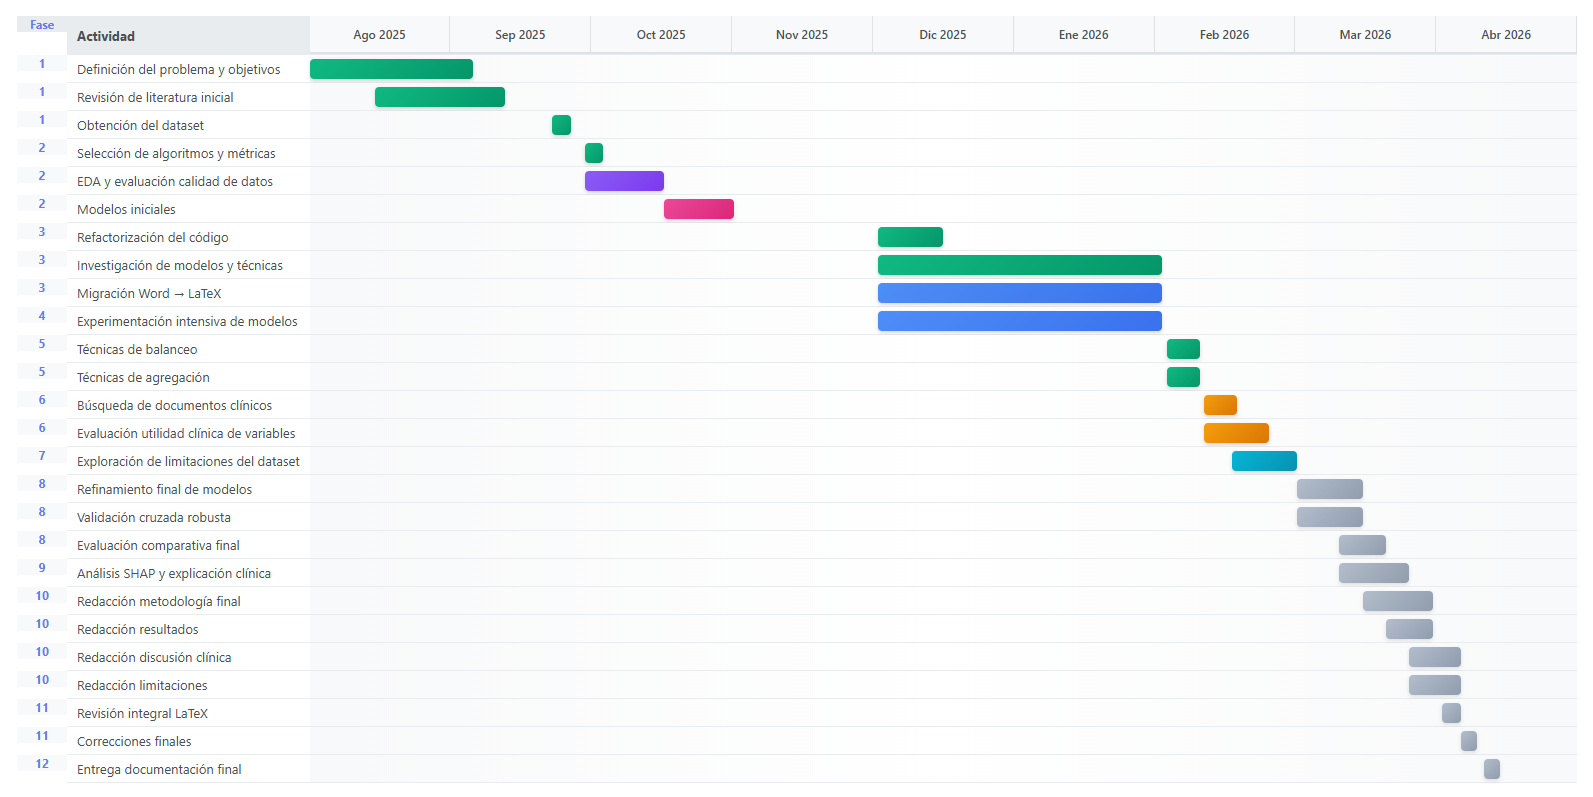
\includegraphics[width=\textwidth]{images/image025.png}
\caption{Cronograma detallado del Proyecto de Grado en Inteligencia Artificial, elaborado mediante TeamGantt}
\end{figure}

\subsection*{Análisis de Participación}
\addcontentsline{toc}{subsection}{Análisis de Participación}

\begin{itemize}
    \item Gustavo Adolfo Cruz Suarez -- Médico Anestesiólogo (FVL)
    \item Daniela Hincapié -- Médico Centro de Investigaciones Clínicas (FVL)
    \item Felipe Ocampo Osorio -- Director de IA (FVL)
\end{itemize}

\newpage